% !TEX output_directory = ./.temp/manual
% !TEX options = --shell-escape

\documentclass[a4paper, 12pt]{article}
\usepackage[outputdir=./.temp/manual]{common}

\usepackage{caption} % Captions outside floats
\usepackage{array} % Advanced tabular col types
\usepackage{longtable} % Multi-page tables
\usepackage{istgame} % Trees

% Prefix appendices with "Appendix".
\usepackage[titletoc,title]{appendix}

% Overlay text and braces over minted.
\usepackage{tikz}
\usetikzlibrary{tikzmark,decorations.pathreplacing,calligraphy}

% Centre minted.
% https://tex.stackexchange.com/a/161128
\usepackage{xpatch, letltxmacro}
\LetLtxMacro{\cminted}{\minted}
\let\endcminted\endminted
\xpretocmd{\cminted}{\RecustomVerbatimEnvironment{Verbatim}{BVerbatim}{}}{}{}

% https://tex.stackexchange.com/a/5020
\newcolumntype{x}[1]{>{\centering\let\newline\\\arraybackslash\hspace{0pt}}p{#1}}
\newenvironment{funcdefs}
    {\begin{longtable}{@{} x{0.33\linewidth} @{} >{\raggedright\arraybackslash}p{0.66\linewidth} @{}}}
    {\end{longtable}}

\def\specialf/{\textit{Special form}\hspace{0.5em}}

\title{lispy Language Manual}

\begin{document}

\maketitle
{
\hypersetup{linkcolor=black}
\tableofcontents
}

\newpage
\section{Introduction}
\lispy/ is a compiled, statically typed, lexically scoped, and type-inferred LISP-like language. Rather than being based on the more modern and complex dialects of LISP, \lispy/ is based on LISP 1.5, as described in \href{https://www.lispmachine.net/books/LISP_1.5_Programmers_Manual.pdf}{\textit{LISP 1.5 Programmer's Manual}} (McCarthy et al., 1985) and \href{http://www.softwarepreservation.org/projects/LISP/book/Weismann_LISP1.5_Primer_1967.pdf}{\textit{LISP 1.5 Primer}} (Weismann, 1967). However, it has significant adjustments and deviations from LISP 1.5. This helps the language stay small and manageable, but a lot of the differences also stem from the need to make the language statically typed rather than dynamically typed.

\section{S-expressions}
The fundamental syntactic element of the language is the \textit{S-expression}. An S-expression is a branching binary tree structure of an indefinite length. In its simplest form, an S-expression is defined as either an atom or an expression \texttt{(A . B)} where \texttt{A} and \texttt{B} are S-expressions. However, \lispy/ does not support the dot notation for S-expressions; it only supports the list notation e.g. \texttt{(A B)}. This is not equivalent to the previous expression. In the list notation, there is an implicit \texttt{nil} as the last element i.e. it is equivalent to \texttt{(A . (B . nil))}. This has a significant implication in that it's impossible to represent data like \texttt{(A . B)}. In the context of a binary tree, this restriction means that the right leaves are always \texttt{nil}. \texttt{nil} will be discussed in more detail later.

\begin{figure}[htb]
    \centering
    \begin{istgame}
        \setistgrowdirection'{east}
        \setistOvalNodeStyle{.8cm}

        \istrooto'(0){}+{15mm}..{14mm}+
            \istb
            \istb
        \endist

        \xtShowEndPoints[oval node]
        \xtdistance{15mm}{14mm}

        \istrooto(1)(0-1){}
            \istb
            \istb{}{\texttt{5}}[center]
        \endist

        \istrooto(2)(0-2){\texttt{sum}}
        \endist

        \istrooto(3)(1-1){}
            \istb{}{\texttt{nil}}[center]
            \istb
        \endist

        \istrooto(4)(3-2){}
            \istb
            \istb
        \endist

        \istrooto(5)(4-1){}
            \istb
            \istb{}{\texttt{10}}[center]
        \endist

        \istrooto(6)(5-1){}
            \istb{}{\texttt{nil}}[center]
            \istb{}{\texttt{2}}[center]
        \endist

        \istrooto(7)(4-2){\texttt{prod}}
        \endist
    \end{istgame}
    \captionsetup[figure]{font=small}
    \captionof{figure}{A binary tree representation of \texttt{(sum 5 (prod 10 2))}.}
\end{figure}

An \textit{atom}, also knows as an \textit{atomic symbol} can be either numeric, Boolean, or neither. The latter is known as a \textit{literal atom}, and in some contexts is referred to as a \textit{variable}.

There are some syntactic differences from LISP 1.5. First, commas are not valid delimiters for elements in the list notation. Second, atomic symbols can be a mix of upper/lower-case letters, digits, and underscores. These are case-sensitive. Finally, the names of constants and functions built into the language are all in lowercase.

\section{Forms}
As in LISP, computation in \lispy/ is done by evaluating \textit{forms}. Forms are specific kinds of S-expressions, typically involving specific types and arrangements of elements within lists. All forms have value, and the value of the form is the result of evaluating it. Forms have already been mentioned, such as for the bodies of lambdas, and lambda expressions themselves. In \lispy/, there are four kinds of forms: elementary forms, simple forms, composed forms, and special forms.

\subsection{Elementary Forms}
\subsubsection{Variables}
All variables are elementary forms. A \textit{variable} is an atomic literal that is associated with some value. The atomic literal serves as an identifier or name for the value, meaning the atomic literal can be evaluated to get the associated value. Thus, evaluating a variable results in its associated value.

The process of associating a value with an identifier is called \textit{(name) binding}. A pair of a bound identifier and its value is called a \textit{binding}. An identifier can be re-bound i.e. \textit{assigned} a new value. There is further discussion in~\nameref{sec:bindingassign}.

\subsubsection{Constants}
All constants are elementary forms. All numbers are constants. Built-in values such as the Booleans \texttt{true} and \texttt{false} are also constants. The result of evaluating a constant is simply that constant itself. For example, the value of \texttt{2.4} is 2.4.

\subsection{Simple Forms}\label{subsec:simpleforms}
Simple forms consist of a left parenthesis, a function name, 0 or more function arguments, and a right parenthesis. A simple form is used to evaluate a function.

A \textit{function} is a named form that can be re-used in evaluations with different sets of inputs. The form is known as the \textit{body} and the inputs are known as \textit{arguments}. The function is defined with variables known as \textit{parameters}, which are accessible to the body. When a function is \textit{called}, or evaluated, the arguments are bound to the parameters, and the body is evaluated using the bound parameters. The result of evaluation is the \textit{return value}.

\begin{figure}[htp]
    \centering
    \begin{cminted}[autogobble=true, escapeinside=??]{lisp}
        (?\tikzmark{name_start}?sum?\tikzmark{name_end}? ?\tikzmark{args_start}?1 2 3 4?\tikzmark{args_end}?)
    \end{cminted}
    \begin{tikzpicture}[
        remember picture,
        overlay,
        thick,
        font=\scriptsize,
        every node/.style={pos=0.5, black}
    ]
        \draw[decorate, decoration={calligraphic brace, mirror, raise=0.25em, amplitude=3pt}]
            (pic cs:name_start) -- (pic cs:name_end)
            node[below=0.5em]{name};

        \draw[decorate, decoration={calligraphic brace, mirror, raise=0.25em, amplitude=3pt}]
            (pic cs:args_start) -- (pic cs:args_end)
            node[below=0.5em]{arguments};
    \end{tikzpicture}
    \captionsetup[figure]{font=small, skip=2em}
    \captionof{figure}{A simple form.}
\end{figure}

% TODO: built-in term is mentioned here without being defined.
The function name is either a built-in function name or any variable whose value has a type of \texttt{func}. The arguments are 0 or more variables or constants.

\subsubsection{Evaluation}
\begin{enumerate}
    \item The function name is evaluated to a built-in function or a \texttt{func} value.
    \item All arguments are evaluated from left to right.
    \item The function is called with the evaluated arguments.
    \item The value of the simple form is the value of the function called with the arguments.
\end{enumerate}

\subsection{Composed Forms} \label{subsec:composedforms}
Composition of forms is possible, which allows for more complex programs. A \textit{composed form} is a more generalised version of a simple form. Unlike simple forms, each argument can be \textit{any} form (elementary, simple, composed, or special).

\begin{figure}[htp]
    \centering
    \begin{cminted}[autogobble=true, escapeinside=??]{lisp}
        (?\tikzmark{name2_start}?prod?\tikzmark{name2_end}? ?\tikzmark{arg2_start}?(div 4 2) ?\tikzmark{sform_start}?(div 6 2)?\tikzmark{sform_end}??\tikzmark{arg2_end}?)
    \end{cminted}
    \begin{tikzpicture}[
        remember picture,
        overlay,
        thick,
        font=\scriptsize,
        every node/.style={pos=0.5, black}
    ]
        \draw[decorate, decoration={calligraphic brace, mirror, raise=0.25em, amplitude=3pt}]
            (pic cs:name2_start) -- (pic cs:name2_end)
            node[below=0.5em]{function name};

        \draw[decorate, decoration={calligraphic brace, mirror, raise=0.25em, amplitude=3pt}]
            (pic cs:sform_start) -- (pic cs:sform_end)
            node[below=0.5em]{simple form};

        \draw[decorate, decoration={calligraphic brace, mirror, raise=1.75em, amplitude=3pt}]
            (pic cs:arg2_start) -- (pic cs:arg2_end)
            node[below=2em]{arguments};
    \end{tikzpicture}
    \captionsetup[figure]{font=small, skip=3.5em}
    \captionof{figure}{A composed form which evaluates to $(4 \div 2) \times (6 \div 2) = 2 \times 3 = 6$.}
\end{figure}

\subsubsection{Evaluation}
\begin{enumerate}
    \item The function name is evaluated to a built-in function or a \texttt{func} value.
    \begin{enumerate}
        \item If the argument is a constant, the constant itself is the value of the argument.
        \item If the argument is a variable, the associated value is the value of the variable.
        \item If the argument is a simple form, it is evaluated using the previously described process for simple forms.
        \item If the argument is a composed form, the partially evaluated arguments are temporarily saved, and steps 1 to 4 are applied recursively to that composed form.
    \end{enumerate}
    \item The function is called with the evaluated arguments.
    \item The value of the composed form is the value of the function called with the arguments.
\end{enumerate}

However, this is not the complete description of composed forms. The function name can actually be any form which evaluates to a function. Thus, it is more appropriate to call it an expression than a name. This will be shown when discussing the~\nameref{subsec:func} type.

\subsection{Special Forms}
The language has built-in functions that are available to the programmer. Some superficially appear to be like most functions, but are actually treated differently. These functions are known as \textit{special forms}. Special forms differ from regular functions in how they're evaluated or how they're defined. They can generally be categorised into one or more of the following:

\begin{enumerate}
    \item Special forms with an indefinite number of arguments.
    \item Special forms that don't evaluate some or all of their arguments.
    \item Special forms that allow an argument or return value to be more than one type.
\end{enumerate}

Note that these kinds of qualities are not achievable with user-defined functions; special forms are implemented using internal facilities not available to the programmer.
% TODO: Discuss that indef args are implemented by expanding a function to e.g. (cons 1 (cons 2 nil)).

Built-in functions are all accessible through variables. The variables for special forms cannot be assigned new values.

\section{Top-level Program}
The top level may have zero or more S-expressions with any amount of whitespace between them. However, consecutive atoms must be separated by at least one whitespace character.

As an example, given the LISP 1.5 program \texttt{MAX (1 2)}, the equivalent in \lispy/ is \texttt{(max 1 2)}. For those familiar with LISP 1.5, \lispy/ effectively uses \texttt{EVAL} at the top level rather than \texttt{EVALQUOTE}, which makes it more akin to the modern LISP dialects.

\section{Types}
\lispy/ is statically typed. This means type safety (i.e. that there are no discrepancies between expected types of values and actual types of values) is verified at compile time by analysing the source code. The language has  a small set of types and a limited (but simple) type system. The language has type inference for everything except function parameters, meaning it can determine the type of a value at compile time without relying on being explicitly told the type by the programmer.

\subsection{int and float}
There are both integer and rational numbers. The former are \texttt{int}s and the latter are \texttt{float}s (a fixed-point representation). The syntax for them is a bit laxer than it is in LISP 1.5 (see~\nameref{sec:syntax}). However, octal number literals are unsupported. There are also \texttt{float} constants for \texttt{inf} (floating-point positive infinity) and \texttt{nan} (``not a number'').

The behaviour of precision and overflow is implementation-defined. For the reference implementation, these types are implemented using Python's \texttt{int} and \texttt{float} types, so they are subject to the same limitations in \lispy/ as they are in Python. That further depends on the Python interpreter used to run the compiled code.

\subsection{bool}
The \texttt{bool} type is represented by the literal atoms \texttt{true} and \texttt{false}. This is a replacement for the \texttt{T} and \texttt{NIL} used by predicates in LISP 1.5. Having a single Boolean type makes it simple from a type checking perspective to implement predicates in \lispy/.

% TODO: mention that recursion is possible.
\subsection{func} \label{subsec:func}
A \texttt{func} is a function as described in~\nameref{subsec:simpleforms}. The fundamental way to create a function is with a special form know as a \textit{lambda expression}. The resulting function is called a \textit{lambda function}. The distinction from just \textit{function} is that a lambda function is not bound to any name. Thus, to evaluate a lambda function, a composed form has to be used. In fact, the use of a lambda expression in place of a function name is what was being alluded to briefly in the description of~\nameref{subsec:composedforms}. As with function names, the lambda expression is evaluated first in the form, and then the arguments are evaluated.

\begin{figure}[htp]
    \centering
    \begin{cminted}[autogobble=true, escapeinside=??]{lisp}
        (?\tikzmark{exp_start}?(lambda ?\tikzmark{param_start}?((?\tikzmark{atom_start}?x?\tikzmark{atom_end}? int) (y ?\tikzmark{type_start}?int?\tikzmark{type_end}?))?\tikzmark{param_end}? ?\tikzmark{form_start}?(div x y)?\tikzmark{form_end}?)?\tikzmark{exp_end}? ?\tikzmark{arg_start}?1 2?\tikzmark{arg_end}?)
    \end{cminted}
    
\begin{tikzpicture}[
        remember picture,
        overlay,
        thick,
        font=\scriptsize,
        every node/.style={pos=0.5, black}
    ]
        \draw[decorate, decoration={calligraphic brace, mirror, raise=0.25em, amplitude=1pt}]
            (pic cs:atom_start) -- (pic cs:atom_end)
            node[below=0.5em]{atomic literal};

        \draw[decorate, decoration={calligraphic brace, mirror, raise=0.25em, amplitude=3pt}]
            (pic cs:type_start) -- (pic cs:type_end)
            node[below=0.5em]{type};

        \draw[decorate, decoration={calligraphic brace, mirror, raise=1.75em, amplitude=3pt}]
            (pic cs:param_start) -- (pic cs:param_end)
            node[below=2em]{parameters};

        \draw[decorate, decoration={calligraphic brace, mirror, raise=0.25em, amplitude=3pt}]
            (pic cs:form_start) -- (pic cs:form_end)
            node[below=0.5em]{body};

        \draw[decorate, decoration={calligraphic brace, mirror, raise=0.25em, amplitude=3pt}]
            (pic cs:arg_start) -- (pic cs:arg_end)
            node[below=0.5em]{arguments};

        \draw[decorate, decoration={calligraphic brace, mirror, raise=3.25em, amplitude=5pt}]
            (pic cs:exp_start) -- (pic cs:exp_end)
            node[below=3.5em]{lambda expression};
    \end{tikzpicture}
    \captionsetup[figure]{font=small, skip=5em}
    \captionof{figure}{A lambda function being evaluated.}
\end{figure}

A function's evaluated value (the \textit{return value}) is the result of evaluating the function body with the function variables, which are bound to some values (the \textit{arguments}) prior to evaluation.

Function parameters are defined as pairs, of which there can be 0 or more. The first element of the pair is the name of the parameter. The second element is the type of that parameter. All parameters must be specified with their types; they are never type-inferred. Note that neither element of this pair is evaluated (this is possible because a lambda expression is a special form).

Unlike parameters, the return value and arguments \textit{will} be type inferred. In fact, there is no mechanism in the language for explicitly specifying the type of a return value or argument.

\subsubsection{First-class Functions}
Functions are \textit{first-class citizens} in the language. This means that, like other values, a function can be passed as an argument to another function, can be returned from other functions, and can be assigned to variables. As a consequence, \textit{higher-order functions} are supported, which are functions that takes a function as an argument and/or return a function.

\begin{figure}[htp]
    \centering
    \begin{cminted}[autogobble=true]{lisp}
        (lambda ((f (func (int int) int))
                 (i int))
          (f 3 i)
        )
    \end{cminted}
    \captionsetup[figure]{font=small}
    \captionof{figure}{A higher-order function that takes a function \texttt{f} as an argument. \texttt{f} has two \texttt{int} parameters and an \texttt{int} return value.}
\end{figure}

\paragraph{Special Forms}
Unlike regular functions, special forms are not first-class citizens. However, this can be worked around by defining a lambda function which ``wraps'' the special form.

\begin{figure}[htp]
    \centering
    \begin{cminted}[autogobble=true]{lisp}
        ((lambda ((f (func (int int) int))
                 (i int))
          (f 3 i))
        (lambda ((a int) (b int)) (prod a b)) 2)
    \end{cminted}
    \captionsetup[figure]{font=small}
    \captionof{figure}{A lambda function wrapping a special form and being passed to another function. This is effectively doing $3 \times 2 = 6$.}
\end{figure}

\subsubsection{define}
Lambda functions are not inherently bound to any variable. However, it can be quite useful to define a function so it can be re-used later. Since lambda functions are first-class citizens, it is valid to assign a lambda expression to a variable.

One way to do this has actually already been shown: rely on the binding mechanism of a lambda expression. A lambda can be bound to another lambda's parameters, and then the lambda will be accessible via a variable within the other lambda. However, this is tedious. A more convenient way to define functions with names is to use the \texttt{define} special form.

\begin{figure}[htp]
    \centering
    \begin{cminted}[autogobble=true, escapeinside=??]{lisp}
        (define ?$name$? ((x int) (y int))
          (div x y)
        )
    \end{cminted}
    \captionsetup[figure]{font=small}
    \captionof{figure}{The \texttt{define} special form.}
\end{figure}

Later, the special form \texttt{set} will be discussed, which is a more general way of creating variables. \texttt{define} is actually equivalent to \texttt{(set $name$ (lambda $\ldots$))}.

\subsection{list}
The \texttt{list} type stores a homogenous (i.e. all of the same type) sequence of elements. Lists always have \texttt{nil} as the final element.

Lists can be created with the special form \texttt{cons}. For example, \texttt{(cons 1 (2 (3 nil)))} creates the list \texttt{(1 2 3)} (the presence of \texttt{nil} is implicit). Notice that the second argument must be a list which holds elements that have the same type as the first argument. Alternatively, the special form \texttt{list}, which takes an indefinite number of arguments, can create the same list: \texttt{(list 1 2 3)}.

The first element of a list can be retrieved using the special form \texttt{car}. For example, \texttt{(car (list 1 2 3))} returns the value \texttt{1}. Conversely, \texttt{cdr} can be used to retrieve the remaining list: \texttt{(cdr (list 1 2 3))} returns the value \texttt{(2 3)}. Both \texttt{car} and \texttt{cdr} only accept one argument, which must be a \texttt{list}.

\begin{figure}[htp]
    \centering
    \begin{cminted}[autogobble=true]{lisp}
        (lambda ((n int) (l (list int)))
          (prod n (car l)))
    \end{cminted}
    \captionsetup[figure]{font=small}
    \captionof{figure}{A lambda with a parameter that's a \texttt{list} of \texttt{int}s.}
\end{figure}

\subsubsection{nil}
The literal atom \texttt{nil} represents an empty list. Thus, it also has a type of \texttt{list}. In fact, an alternative way to represent \texttt{nil} is \texttt{()}. For \texttt{nil}, \texttt{car} and \texttt{cdr} are unsupported -- attempting to do so will result in a runtime error.

\texttt{nil} is a built-in ``global'' variable that's accessible everywhere. However, it's special as far as variables go because it cannot be assigned a new value.

\section{Conditional Expressions}
A \textit{conditional expression} is a special form that can branch evaluation conditionally on the value of forms. \lispy/ has two special forms for conditional expressions: \texttt{cond} and \texttt{select}.

\subsection{cond}

\texttt{cond} has one or more pairs of a predicate $p_i$ and a form $e_i$ followed by a single form $e$ at the end. A \textit{predicate} is a form that evaluates to a \texttt{bool}. All forms $e_1 \ldots e_n$ and $e$ must evaluate to the same type.

\begin{figure}[htp]
    \centering
    \begin{cminted}[autogobble=true, escapeinside=??]{lisp}
        (cond (?$p_1$? ?$e_1$?) (?$p_2$? ?$e_2$?) ?$\ldots$? (?$p_n$? ?$e_n$?) ?$e$?)
    \end{cminted}
    \captionsetup[figure]{font=small}
    \captionof{figure}{The \texttt{cond} special form.}
\end{figure}

From left to right, the predicate of each pair is evaluated. If $p_i$ evaluates to \texttt{true}, then $e_i$ is evaluated and returned from \texttt{cond}; no further evaluation is performed. Otherwise, $e_i$ is not evaluated and the evaluation step is repeated using $p_{i + 1}$ until $p_n$. If all predicates are \texttt{false}, the form $e$ is evaluated and returned, making it a default value for the conditional expression.

% TODO: maybe add a concrete example of using cond?

\subsection{select}

\texttt{select} has a form $p$ followed by one or more pairs of forms $(p_i\ e_i)$ and ends with a form $e$. All forms $p$ and $p_1 \ldots p_n$ must evaluate to the same type. Furthermore, all forms $e_1 \ldots e_n$ and $e$ must evaluate to the same type.

\begin{figure}[htp]
    \centering
    \begin{cminted}[autogobble=true, escapeinside=??]{lisp}
        (select ?$p$? (?$p_1$? ?$e_1$?) (?$p_2$? ?$e_2$?) ?$\ldots$? (?$p_n$? ?$e_n$?) ?$e$?)
    \end{cminted}
    \captionsetup[figure]{font=small}
    \captionof{figure}{The \texttt{select} special form.}
\end{figure}

First, $p$ is evaluated once and its value is temporarily stored. From left to right, $p_i$ is evaluated and compared to the value of $p$ using the built-in predicate \texttt{equal}. If this comparison evaluates to \texttt{true}, then $e_i$ is evaluated and returned from \texttt{select}; no further evaluation is performed. Otherwise, $e_i$ is not evaluated and the evaluation step is repeated used $p_{i + 1}$ until $p_n$. If no equality is found, then $e$ is evaluated and returned, making it a default value for the conditional expression.

Due to the use of \texttt{equal}, $p$ must not be a \texttt{func} or a \texttt{list} which contains a \texttt{func} at the top level or in any nested list.

\section{Evaluating Multiple Forms}
The body of a lambda can be any form, including composed forms. This means the lambda can evaluate multiple forms by continuously nesting lambdas within its body. While this is very useful, it is quite tedious. The special form \texttt{progn} solves this by taking 2 or more forms as arguments, evaluating all forms, and returning the value of the last form.

\begin{figure}[htp]
    \centering
    \begin{cminted}[autogobble=true, escapeinside=??]{lisp}
        (progn ?$e_1$? ?$e_2$? ?$\ldots$? ?$e_n$?)
    \end{cminted}
    \captionsetup[figure]{font=small}
    \captionof{figure}{The \texttt{progn} special form.}
\end{figure}

The forms are evaluated left to right, from $e_1$ to $e_n$. The return value of \texttt{progn} is the value of $e_n$. Because only the value of $e_n$ is used, each form may evaluate to a different type.
% TODO: show how progn translates to chained lambdas.

\section{Binding}\label{sec:bindingassign}
Recall that variables can be bound to values, and existing variables can be assigned new values. This section deals with how these operations are performed in the language.

But first, clarification is needed on what constitutes a valid name for a binding. Generally, a valid name is any atomic literal. This means numbers and the Boolean constants \texttt{true} and \texttt{false} are not valid names. Special forms cannot be assigned new values. However, built-in function names (including special form names) can be used as names for new bindings. This results in \textit{shadowing}, a subject explained in~\nameref{sec:scope}.

\subsection{let}
A way to bind variables was introduced with lambda expressions. However, as with the problem \texttt{progn} solves, writing lambdas for this becomes tedious. Instead, the special form \texttt{let} can be used to bind variables. It can be thought of as a more powerful version of \texttt{progn}.

\begin{figure}[htp]
    \centering
    \begin{cminted}[autogobble=true, escapeinside=??]{lisp}
        (let ((?$a_1$? ?$d_1$?) (?$a_2$? ?$d_2$?) ?$\ldots$? (?$a_n$? ?$d_n$?)) ?$e_1$? ?$e_2$? ?$\ldots$? ?$e_n$?)
    \end{cminted}
    \captionsetup[figure]{font=small}
    \captionof{figure}{The \texttt{let} special form.}
\end{figure}

\texttt{let} has one or more pairs of bindings $(a_i\ d_i)$ followed by one or more forms $e_1 \ldots e_n$. The forms $e_1 \ldots e_n$, collectively known as the \textit{body}, have the same semantics as in \texttt{progn}, except for the benefit of also having access to the variable bindings that precede them. The binding is performed left to right from $(a_1\ d_1)$ to $(a_n\ d_n)$. $d_i$ is the form to evaluate and bind to $a_i$, which is the name of the variable. Just like in lambda expressions, the variable name $a_i$ is not evaluated. As with \texttt{progn}, \texttt{let} returns the value of the last form, $e_n$.

The bindings are performed in parallel, meaning $d_i$ cannot use any of $a_1 \ldots a_n$.

\begin{figure}[htp]
    \centering
    \begin{cminted}[autogobble=true]{lisp}
        (let ((a 2) (b (prod a 2))) b)
    \end{cminted}
    \captionsetup[figure]{font=small}
    \captionof{figure}{An invalid use of bindings in \texttt{let}; \texttt{a} cannot be used for \texttt{b}'s definition.}
\end{figure}

Notice that each variable must have an initial value it's bound to. Because of this requirement, it is possible to infer the type of each variable. Hence, there is no need (nor is there a way) to explicitly specify the type of each variable.
% TODO: show how let translates to a lambda that is immediately called.

\subsection{set}
The special form \texttt{set} is a simpler way to create a single binding. It can also be used to assign a new value to a variable.

\begin{figure}[htp]
    \centering
    \begin{cminted}[autogobble=true, escapeinside=??]{lisp}
        (set ?$name$? ?$value$?)
    \end{cminted}
    \captionsetup[figure]{font=small}
    \captionof{figure}{The \texttt{set} special form.}
\end{figure}

$name$ and $value$ are similar to the binding pairs of \texttt{let}. $name$ can either be the name of a new variable, or the name of an existing variable that is currently accessible. In the former case, a new binding is created. In the latter case, the variable is rebound to the new value, and the value must have the same type as value being overwritten. \texttt{set} returns $value$.

Unlike \texttt{let}, \texttt{set} doesn't have any following forms that have access to the binding. So, from where will this new binding be accessible? This is discussed in the following section on scope.

\section{Scope} \label{sec:scope}
An important aspect of binding is understanding where that binding is valid i.e. its scope. A binding is said to be \textit{valid} if the binding's name is considered to be associated with the binding's value in the current part of the program. In other parts, the same name may be bound to a different value or not bound at all. A \textit{scope} is the set of all bindings that are valid within a particular context (part) of the whole program.

\paragraph{Lexical Scope and Context}
\lispy/ is \textit{lexically scoped}, meaning a bound name is resolved based on where the binding was defined. Thus, a ``particular context'' is specifically a lexical context. Generally, a \textit{lexical context} is the boundary of a \textit{lexical unit}. For the discussion of scope, the lexical units that need to be considered are a \texttt{let} expression, a function body, and the whole program.

\paragraph{Nested Scopes}
A scope can be nested within another scope. A nested scope inherits the bindings of its enclosing scope. Resolution of a bound name is first attempted in the local lexical context. If it fails to find the binding in the local lexical context, then it tries again with the outer lexical context. This is repeated until the outer-most lexical context is reached. Past that, a name is considered to be unbound, and a compiler error occurs.

A variable may be defined using a name that already has a binding in an outer scope. This variable \textit{shadows} the one in the outer scope; according to the name resolution algorithm just described, the inner binding has precedence over the outer binding.

\subsection{Scope Levels}
There are three levels of scope: global scope, function scope, and expression scope.

\paragraph{Global}
Global scope is the top level of the program. There is only one global scope, and all other scopes are nested within the global scope. Built-in functions are in the global scope.

\paragraph{Function}
In a function scope, a binding defined within a function does not extend outside of that function. With lexical scoping, a binding only has scope within the lexical context of the function i.e. the boundaries of that function's definition. This means that if the function calls another function, the bindings go out of context (because the other function is defined elsewhere); the bindings cannot be accessed from the called function. When that called function returns, the bindings come back into context.

\paragraph{Expression}
In an expression scope, a binding has scope within the lexical context of that expression (again, this is lexical scoping). As with functions, bindings go out of context when other functions are called and come back into context when that called function returns. Thus, in a \texttt{let} expression, the initial bindings (the $(a_i\ d_i)$ pairs) are accessible to all forms in the body, but not outside the \texttt{let} expression.

\subsection{set}
\texttt{set} can create a new binding or rebind an existing variable. When a new binding is created by \texttt{set}, the scope of that binding is the enclosing scope of the \texttt{set} call. It is not possible to create a binding that has a more outer scope.

\begin{figure}[htp]
    \centering
    \begin{cminted}[autogobble=true, escapeinside=??]{lisp}
        (lambda (a) (progn (set b 2) (prod a b)))
    \end{cminted}
    \captionsetup[figure]{font=small}
    \captionof{figure}{The scope of \texttt{b} is the scope of the enclosing lambda function; \texttt{a} and \texttt{b} have the same scope.}
\end{figure}

For \texttt{set} to rebind an existing variable, that variable has to be in an enclosing scope of the \texttt{set} call i.e. it should be possible to resolve that name as described earlier. Otherwise, the name is considered unbound, and a new binding within the enclosing scope is created instead.

\subsection{Closures}
Nested functions complicate the matter. First, because a nested function is defined within the local lexical context, calling it does not cause bindings to go out of context. The nested function will have access to its own bindings and those of its enclosing scope. However, the enclosing scope will not have access to the nested function's bindings.

Second, because functions are first-class citizens, they can be returned and called from other contexts. This means the compiler must create a closure to store copies of the required non-local variables (names that only resolve in an enclosing context). A \textit{closure} is a pair of a function and the set of non-local variables that are used within the function. Thus, even if the function is called outside its defined context, it will have access to all the variables it depends on.

\section{Built-in Functions}
First, recall the following built-ins, which have already been presented and will not be discussed any further in this section:
\begin{center}
    \texttt{%
    \begin{tabular}{l l l l}
        list & cons & car & cdr \\
        cond & select & let & set \\
        lambda & progn
    \end{tabular}}
\end{center}

While discussing functions here, all arguments can be assumed to be evaluated unless explicitly noted otherwise. For example, stating an argument $a$ must be a \texttt{bool} really means that it must be some form that evaluates to a \texttt{bool}. Furthermore, all arguments can be assumed to be evaluated left to right unless explicitly noted otherwise. Finally, recall that a special form is not a first-class citizen, so it cannot be used as an argument (but it can be called so that its return value is used as an argument).

\pagebreak[4] % CLEANUP
\subsection{Predicate Functions}
\begin{funcdefs}
    \begin{minipage}[t]{\linewidth}
        \centering
        \begin{cminted}[autogobble=true, escapeinside=??]{lisp}
            (eq ?$e_1$? ?$e_2$?)
        \end{cminted}
    \end{minipage}
    & \specialf/ Returns \texttt{true} if the values of $e_1$ and $e_2$ have the same internal memory address. Otherwise, returns \texttt{false}. The values must be of the same type. The values cannot be \texttt{int}s, \texttt{float}s, or special forms. This is always \texttt{true} if both arguments are \texttt{true} or \texttt{false}.
    \\ \\
    \begin{minipage}[t]{\linewidth}
        \centering
        \begin{cminted}[autogobble=true, escapeinside=??]{lisp}
            (equal ?$e_1$? ?$e_2$?)
        \end{cminted}
    \end{minipage}
    & \specialf/ Returns \texttt{true} if the values of $e_1$ and $e_2$ are equivalent. Otherwise, returns \texttt{false}. The values must be of the same type. The values must not be \texttt{func}s.
    \setlength{\parindent}{1.5em}%
    \par\indent%
    \texttt{int}s are equivalent following the rules of mathematics. \texttt{float}s are similar, except that due to a lack of infinite precision, they're equivalent if they're within an implementation-defined distance of each other.
    \par\indent%
    \texttt{list}s are compared element-wise (sensitive to ordering), recursing into nested lists if needed. Lists of differing lengths are trivially not equivalent. Lists must not contain a \texttt{func} at either the top level or in any nested list.
    \par\indent%
    For the Booleans, \texttt{true} is trivially only equivalent to itself and so is \texttt{false}.
\end{funcdefs}
% NOTE: float comparison https://stackoverflow.com/a/32334103
% TODO: should this work differently for nil?

\subsubsection{Arithmetic Predicates}
\begin{funcdefs}
    \begin{minipage}[t]{\linewidth}
        \centering
        \begin{cminted}[autogobble=true, escapeinside=??]{lisp}
            (greaterp ?$n_1$? ?$n_2$?)
        \end{cminted}
    \end{minipage}
    & \specialf/ Returns \texttt{true} if $n_1 > n_2$. Otherwise, returns \texttt{false}. Both arguments must be \texttt{int}s or \texttt{float}s. However, they do not have to the same type; an \texttt{int} can be compared to a \texttt{float}.
    \\ \\
    \begin{minipage}[t]{\linewidth}
        \centering
        \begin{cminted}[autogobble=true, escapeinside=??]{lisp}
            (evenp ?$n$?)
        \end{cminted}
    \end{minipage}
    & Returns \texttt{true} if $n$ is an even number. Otherwise, returns \texttt{false}. $n$ must be an \texttt{int}.
    \\ \\
    \begin{minipage}[t]{\linewidth}
        \centering
        \begin{cminted}[autogobble=true, escapeinside=??]{lisp}
            (lessp ?$n_1$? ?$n_2$?)
        \end{cminted}
    \end{minipage}
    & \specialf/ Returns \texttt{true} if $n_1 < n_2$. Otherwise, returns \texttt{false}. Both arguments must be \texttt{int}s or \texttt{float}s. However, they do not have to the same type; an \texttt{int} can be compared to a \texttt{float}.
\end{funcdefs}

\subsubsection{List Predicates}
\begin{funcdefs}
    \begin{minipage}[t]{\linewidth}
        \centering
        \begin{cminted}[autogobble=true, escapeinside=??]{lisp}
            (null ?$l$?)
        \end{cminted}
    \end{minipage}
    & \specialf/ Returns \texttt{true} if $l$ is \texttt{nil}. Otherwise, returns \texttt{false}. $l$ must be a \texttt{list}. Equivalent to \texttt{(equal $l$ nil)}.
    \\ \\
    \begin{minipage}[t]{\linewidth}
        \centering
        \begin{cminted}[autogobble=true, escapeinside=??]{lisp}
            (member ?$e$? ?$l$?)
        \end{cminted}
    \end{minipage}
    & \specialf/ Returns \texttt{true} $e$ is an element of a list $l$. Otherwise, returns \texttt{false}. $l$ must be a \texttt{list} and $e$ must have the same type as $l$'s elements (except for the implicit terminating \texttt{nil}).
    \setlength{\parindent}{1.5em}%
    \par\indent%
    $e$ is said to be an element of a list $l$ of length $n$ if \texttt{(equal $e$ $l_i$)} is \texttt{true} for any $i$ in $[1, n]$.
\end{funcdefs}

\subsubsection{Logical Connectives}
\begin{funcdefs}
    \begin{minipage}[t]{\linewidth}
        \centering
        \begin{cminted}[autogobble=true, escapeinside=??]{lisp}
            (not ?$p$?)
        \end{cminted}
    \end{minipage}
    & Returns \texttt{true} if $p$ is \texttt{false}. Otherwise, returns \texttt{false}. $p$ must be a \texttt{bool}. Equivalent to \texttt{(eq $p$ true)}.
    \\ \\
    \begin{minipage}[t]{\linewidth}
        \centering
        \begin{cminted}[autogobble=true, escapeinside=??]{lisp}
            (and ?$e_1$? ?$e_2$? ?$\ldots$? ?$e_n$?)
        \end{cminted}
    \end{minipage}
    & \specialf/ Returns \texttt{true} if all $e_1 \ldots e_n$ are \texttt{true}. Otherwise, returns \texttt{false}. $e_1 \ldots e_n$ must all be \texttt{bool}s.
    \\ \\
    \begin{minipage}[t]{\linewidth}
        \centering
        \begin{cminted}[autogobble=true, escapeinside=??]{lisp}
            (or ?$e_1$? ?$e_2$? ?$\ldots$? ?$e_n$?)
        \end{cminted}
    \end{minipage}
    & \specialf/ Returns \texttt{true} if any of $e_1 \ldots e_n$ are \texttt{true}. Otherwise, returns \texttt{false}. $e_1 \ldots e_n$ must all be \texttt{bool}s.
\end{funcdefs}

\noindent \texttt{and} and \texttt{or} don't always evaluate all arguments. When a \texttt{false} argument is encountered for \texttt{and}, the evaluation ends early and the rest of the arguments remain unevaluated. When a \texttt{true} argument is encountered for \texttt{or}, the evaluation ends early and the rest of the arguments remain unevaluated.

\subsection{Arithmetic Functions}
The arithmetic functions only accept numeric types (\texttt{int} and \texttt{float}) as arguments. However, the arguments do not have to be homogenous in type. If there is at least one \texttt{float}, then an arithmetic function returns a \texttt{float}. Otherwise, it returns an \texttt{int}. If the initial result of the computation is not of the right type, then it will be implicitly converted using the \texttt{trunc} and \texttt{float} functions described in the next section.

A runtime error occurs when calling any of these functions with arguments outside the domain of the equivalent mathematical function e.g. division by zero.

\begin{funcdefs}
    \begin{minipage}[t]{\linewidth}
        \centering
        \begin{cminted}[autogobble=true, escapeinside=??]{lisp}
            (sum ?$x_1$? ?$x_2$? ?$\ldots$? ?$x_n$?)
        \end{cminted}
    \end{minipage}
    & \specialf/ Returns $\sum_{i}^{n}{x_i}$, the sum of all arguments. There must be at least two arguments.
    \\ \\
    \begin{minipage}[t]{\linewidth}
        \centering
        \begin{cminted}[autogobble=true, escapeinside=??]{lisp}
            (prod ?$x_1$? ?$x_2$? ?$\ldots$? ?$x_n$?)
        \end{cminted}
    \end{minipage}
    & \specialf/ Returns $\prod_{i}^{n}{x_i}$, the product of all arguments. There must be at least two arguments.
    \\ \\
    \begin{minipage}[t]{\linewidth}
        \centering
        \begin{cminted}[autogobble=true, escapeinside=??]{lisp}
            (diff ?$x$? ?$y$?)
        \end{cminted}
    \end{minipage}
    & \specialf/ Returns $x - y$, the difference of $x$ and $y$.
    \\ \\
    \begin{minipage}[t]{\linewidth}
        \centering
        \begin{cminted}[autogobble=true, escapeinside=??]{lisp}
            (neg ?$x$?)
        \end{cminted}
    \end{minipage}
    & \specialf/ Returns $-x$, the negation of $x$.
    \\ \\
    \begin{minipage}[t]{\linewidth}
        \centering
        \begin{cminted}[autogobble=true, escapeinside=??]{lisp}
            (inc ?$x$?)
        \end{cminted}
    \end{minipage}
    & \specialf/ Returns $x + 1$, $x$ incremented by 1.
    \\ \\
    \begin{minipage}[t]{\linewidth}
        \centering
        \begin{cminted}[autogobble=true, escapeinside=??]{lisp}
            (dec ?$x$?)
        \end{cminted}
    \end{minipage}
    & \specialf/ Returns $x - 1$, $x$ decremented by 1.
    \\ \\
    \begin{minipage}[t]{\linewidth}
        \centering
        \begin{cminted}[autogobble=true, escapeinside=??]{lisp}
            (div ?$x$? ?$y$?)
        \end{cminted}
    \end{minipage}
    & \specialf/ Returns $x / y$, a single number that is the result of division with remainder.
    \\ \\
    \begin{minipage}[t]{\linewidth}
        \centering
        \begin{cminted}[autogobble=true, escapeinside=??]{lisp}
            (mod ?$x$? ?$y$?)
        \end{cminted}
    \end{minipage}
    & \specialf/ Returns $x - y$trunc$(\frac{x}{y})$, the remainder of dividing $x$ by $y$ through truncated division. This is the modulo operation.
    \\ \\
    \begin{minipage}[t]{\linewidth}
        \centering
        \begin{cminted}[autogobble=true, escapeinside=??]{lisp}
            (expt ?$x$? ?$y$?)
        \end{cminted}
    \end{minipage}
    & \specialf/ Returns $x^y$, $x$ to the power of $y$.
    \\ \\
    \begin{minipage}[t]{\linewidth}
        \centering
        \begin{cminted}[autogobble=true, escapeinside=??]{lisp}
            (sqrt ?$x$?)
        \end{cminted}
    \end{minipage}
    & \specialf/ Returns $\sqrt{x}$, the square root of $x$.
    \\ \\
    \begin{minipage}[t]{\linewidth}
        \centering
        \begin{cminted}[autogobble=true, escapeinside=??]{lisp}
            (log ?$x$? ?$y$?)
        \end{cminted}
    \end{minipage}
    & \specialf/ Returns $\log_{y}{x}$, the logarithm of $x$ to base $y$.
    \\ \\
    \begin{minipage}[t]{\linewidth}
        \centering
        \begin{cminted}[autogobble=true, escapeinside=??]{lisp}
            (lb ?$x$?)
        \end{cminted}
    \end{minipage}
    & \specialf/ Returns $\log_{2}{x}$, the binary logarithm of $x$.
    \\ \\
    \begin{minipage}[t]{\linewidth}
        \centering
        \begin{cminted}[autogobble=true, escapeinside=??]{lisp}
            (lg ?$x$?)
        \end{cminted}
    \end{minipage}
    & \specialf/ Returns $\log_{10}{x}$, the common logarithm of $x$.
    \\ \\
    \begin{minipage}[t]{\linewidth}
        \centering
        \begin{cminted}[autogobble=true, escapeinside=??]{lisp}
            (ln ?$x$?)
        \end{cminted}
    \end{minipage}
    & \specialf/ Returns $\log_{\mathrm{e}}{x}$, the natural logarithm of $x$.
    \\ \\
    \begin{minipage}[t]{\linewidth}
        \centering
        \begin{cminted}[autogobble=true, escapeinside=??]{lisp}
            (recip ?$x$?)
        \end{cminted}
    \end{minipage}
    & \specialf/ Returns $\frac{1}{x}$, the reciprocal of $x$.
    \\ \\
    \begin{minipage}[t]{\linewidth}
        \centering
        \begin{cminted}[autogobble=true, escapeinside=??]{lisp}
            (abs ?$x$?)
        \end{cminted}
    \end{minipage}
    & \specialf/ Returns $|x|$, the absolute value of $x$.
    \\ \\
    \begin{minipage}[t]{\linewidth}
        \centering
        \begin{cminted}[autogobble=true, escapeinside=??]{lisp}
            (min ?$x_1$? ?$x_2$? ?$\ldots$? ?$x_n$?)
        \end{cminted}
    \end{minipage}
    & \specialf/ Returns the smallest value in $x_1 \ldots x_n$. There must be at least two arguments. Note that even if the smallest value is an \texttt{int}, it will be returned as a \texttt{float} if there's at least one other argument that is a \texttt{float}.
    \\ \\
    \begin{minipage}[t]{\linewidth}
        \centering
        \begin{cminted}[autogobble=true, escapeinside=??]{lisp}
            (max ?$x_1$? ?$x_2$? ?$\ldots$? ?$x_n$?)
        \end{cminted}
    \end{minipage}
    & \specialf/ Returns the largest value in $x_1 \ldots x_n$. There must be at least two arguments. Note that even if the largest value is an \texttt{int}, it will be returned as a \texttt{float} if there's at least one other argument that is a \texttt{float}.
\end{funcdefs}

\subsection{Numeric Conversion Functions}
\begin{funcdefs}
    \begin{minipage}[t]{\linewidth}
        \centering
        \begin{cminted}[autogobble=true, escapeinside=??]{lisp}
            (float ?$x$?)
        \end{cminted}
    \end{minipage}
    & Returns the \texttt{float} equivalent of an \texttt{int} $x$. For example, \texttt{(float 3)} is $3.0$.
    \\ \\
    \begin{minipage}[t]{\linewidth}
        \centering
        \begin{cminted}[autogobble=true, escapeinside=??]{lisp}
            (floor ?$x$?)
        \end{cminted}
    \end{minipage}
    & Returns $\lfloor x \rfloor$. $x$ must be a \texttt{float}.
    \\ \\
    \begin{minipage}[t]{\linewidth}
        \centering
        \begin{cminted}[autogobble=true, escapeinside=??]{lisp}
            (ceil ?$x$?)
        \end{cminted}
    \end{minipage}
    & Returns $\lceil x \rceil$. $x$ must be a \texttt{float}.
    \\ \\
    \begin{minipage}[t]{\linewidth}
        \centering
        \begin{cminted}[autogobble=true, escapeinside=??]{lisp}
            (trunc ?$x$?)
        \end{cminted}
    \end{minipage}
    & Returns the \texttt{float} $x$ truncated to an \texttt{int}. This rounds towards 0, so $-1.5$ becomes $-1$ and $1.5$ becomes $1$.
    \\ \\
    \begin{minipage}[t]{\linewidth}
        \centering
        \begin{cminted}[autogobble=true, escapeinside=??]{lisp}
            (round ?$x$?)
        \end{cminted}
    \end{minipage}
    & Returns the \texttt{float} $x$ rounded to the nearest \texttt{int}. If $x$ is exactly halfway, then it rounds towards the even choice. For example, $0.5$ and $-0.5$ round to $0$, and $1.5$ rounds to 2.
\end{funcdefs}

\subsection{Bit-wise Functions}
The following functions only accept \texttt{int}s as arguments.
\begin{funcdefs}
    \begin{minipage}[t]{\linewidth}
        \centering
        \begin{cminted}[autogobble=true, escapeinside=??]{lisp}
            (logand ?$x$? ?$y$?)
        \end{cminted}
    \end{minipage}
    & Returns $x \wedge y$, the bit-wise AND of $x$ and $y$.
    \\ \\
    \begin{minipage}[t]{\linewidth}
        \centering
        \begin{cminted}[autogobble=true, escapeinside=??]{lisp}
            (logior ?$x$? ?$y$?)
        \end{cminted}
    \end{minipage}
    & Returns $x \lor y$, the bit-wise OR of $x$ and $y$.
    \\ \\
    \begin{minipage}[t]{\linewidth}
        \centering
        \begin{cminted}[autogobble=true, escapeinside=??]{lisp}
            (logxor ?$x$? ?$y$?)
        \end{cminted}
    \end{minipage}
    & Returns $x \oplus y$, the bit-wise EXCLUSIVE OR of $x$ and $y$.
    \\ \\
    \begin{minipage}[t]{\linewidth}
        \centering
        \begin{cminted}[autogobble=true, escapeinside=??]{lisp}
            (lognot ?$x$? ?$y$?)
        \end{cminted}
    \end{minipage}
    & Returns $\lnot x$, the bit-wise NOT of $x$.
    \\ \\
    \begin{minipage}[t]{\linewidth}
        \centering
        \begin{cminted}[autogobble=true, escapeinside=??]{lisp}
            (shift ?$x$? ?$y$?)
        \end{cminted}
    \end{minipage}
    & Returns $x$ arithmetically shifted by $y$ bits. If $y$ is positive, $x$ is shifted to the left. If $y$ is negative, $x$ is shifted to the right.
\end{funcdefs}

\subsection{List Functions}
\begin{funcdefs}
    \begin{minipage}[t]{\linewidth}
        \centering
        \begin{cminted}[autogobble=true, escapeinside=??]{lisp}
            (append ?$e$? ?$l$?)
        \end{cminted}
    \end{minipage}
    & \specialf/ Returns copy of the \texttt{list} $l$ with a new element $e$ at the end of it (it is still terminated with \texttt{nil}). The copy behaves like the built-in \texttt{copy} function. $e$ must have the same type as the elements of $l$.
    \\ \\
    \begin{minipage}[t]{\linewidth}
        \centering
        \begin{cminted}[autogobble=true, escapeinside=??]{lisp}
            (extend ?$l_1$? ?$l_2$?)
        \end{cminted}
    \end{minipage}
    & \specialf/ Returns a new \texttt{list} which is the combination of the elements of the \texttt{list}s $l_1$ and $l_2$. The elements are copied in order like with the built-in \texttt{copy} function. The elements of $l_2$ follow those of $l_1$. $l_1$ and $l_2$ must have the same type.
    \\ \\
    \begin{minipage}[t]{\linewidth}
        \centering
        \begin{cminted}[autogobble=true, escapeinside=??]{lisp}
            (copy ?$l$?)
        \end{cminted}
    \end{minipage}
    & \specialf/ Returns a shallow copy of the \texttt{list} $l$. In a shallow copy, all the top-level elements are copied, but any nested lists are not recursively copied. Thus, for some list \texttt{A}, \texttt{B = (list A)}, and \texttt{C = (copy B)}, \texttt{(eq C B)} is \texttt{false}, \texttt{(equal C B)} is \texttt{true}, and \texttt{(eq (car C) A)} is \texttt{true}.
    \\ \\
    \begin{minipage}[t]{\linewidth}
        \centering
        \begin{cminted}[autogobble=true, escapeinside=??]{lisp}
            (reverse ?$l$?)
        \end{cminted}
    \end{minipage}
    & \specialf/ Returns a new \texttt{list} which contains the elements of \texttt{list} $l$ in reversed order. Only the top-level elements are reversed; nested keep their internal order. \texttt{nil} is excluded from the reversal and is still at the end to terminate the new list.
    \\ \\
    \begin{minipage}[t]{\linewidth}
        \centering
        \begin{cminted}[autogobble=true, escapeinside=??]{lisp}
            (length ?$l$?)
        \end{cminted}
    \end{minipage}
    & \specialf/ Returns an \texttt{int} which is the number of items in the \texttt{list} $l$. The terminating \texttt{nil} is not counted towards the length, and \texttt{(length nil)} is 0.
    \\ \\
    \begin{minipage}[t]{\linewidth}
        \centering
        \begin{cminted}[autogobble=true, escapeinside=??]{lisp}
            (efface ?$e$? ?$l$?)
        \end{cminted}
    \end{minipage}
    & \specialf/ Returns a copy of the \texttt{list} $l$ with the first occurrence of the element $e$ removed. $e$ must have the same type as the elements of $l$. Elements are compared using the built-in \texttt{equal} function, so $e$ must not be a \texttt{func} or a \texttt{list} which contains a \texttt{func} at the top level or in any nested list. The copy behaves like the built-in \texttt{copy} function.
\end{funcdefs}

\subsection{Input and Output}
Values can be \textit{printed} i.e. written to the standard output (\textit{stdout}). However, input is not supported. Values are output using their S-expression representation. The exception to this is functions, which are output as ``<function at \textit{memory-address}>''. Special forms cannot be printed.

\begin{funcdefs}
    \begin{minipage}[t]{\linewidth}
        \centering
        \begin{cminted}[autogobble=true, escapeinside=??]{lisp}
            (print ?$e_1$? ?$e_2$? ?$\ldots$? ?$e_n$?)
        \end{cminted}
    \end{minipage}
    & \specialf/ Prints a single line of all arguments concatenated with a space delimiter. The arguments do not need to be homogenous in type. Zero arguments may be given, in which case only a single space character is printed. Returns \texttt{nil}.
    \\ \\
    \begin{minipage}[t]{\linewidth}
        \centering
        \begin{cminted}[autogobble=true, escapeinside=??]{lisp}
            (println ?$e_1$? ?$e_2$? ?$\ldots$? ?$e_n$?)
        \end{cminted}
    \end{minipage}
    & \specialf/ Similar to \texttt{print} except that the line is also terminated with a newline character. Zero arguments may be given, in which case only a single newline character is printed.
\end{funcdefs}

\subsection{Mapping Functions}
\begin{funcdefs}
    \begin{minipage}[t]{\linewidth}
        \centering
        \begin{cminted}[autogobble=true, escapeinside=??]{lisp}
            (map ?$l$? ?$f$?)
        \end{cminted}
    \end{minipage}
    & \specialf/ Returns a \texttt{list} of the results of applying the function $f$ to the list $l$ and to successive \texttt{(cdr $l$)} until $l$ is reduced to \texttt{nil}. $f$ must be a \texttt{func} with a single parameter whose type matches the type of the elements of \texttt{list} $l$.
    \\ \\
    \begin{minipage}[t]{\linewidth}
        \centering
        \begin{cminted}[autogobble=true, escapeinside=??]{lisp}
            (mapcar ?$l$? ?$f$?)
        \end{cminted}
    \end{minipage}
    & \specialf/ Returns a \texttt{list} of the results of applying the function $f$ to each element of the list $l$, excluding the terminating \texttt{nil}. $f$ must be a \texttt{func} with a single parameter whose type matches the type of the elements of \texttt{list} $l$.
\end{funcdefs}

\newpage
\begin{appendices}
    \section{Syntax}\label{sec:syntax}
    \subsection{Abstract}
    \textit{Note:} \texttt{*} denotes zero or more of the preceding term. \texttt{+} denotes one or more of the preceding term.
    \inputminted[fontsize=\footnotesize, samepage]{bnf}{grammar_abstract.bnf}

    \subsection{Concrete}
    \inputminted[fontsize=\footnotesize, samepage]{ebnf}{grammar.ebnf}
\end{appendices}

\end{document}
